% !TeX root = ../libro.tex
% !TeX encoding = utf8

\chapter{Resultado de técnicas empleadas al renderizar SDFs}\label{ap:comparacionEscenas}

\begin{figure}[ht!]
    \centering
    \begin{subfigure}[b]{0.3\textwidth}
        \centering
        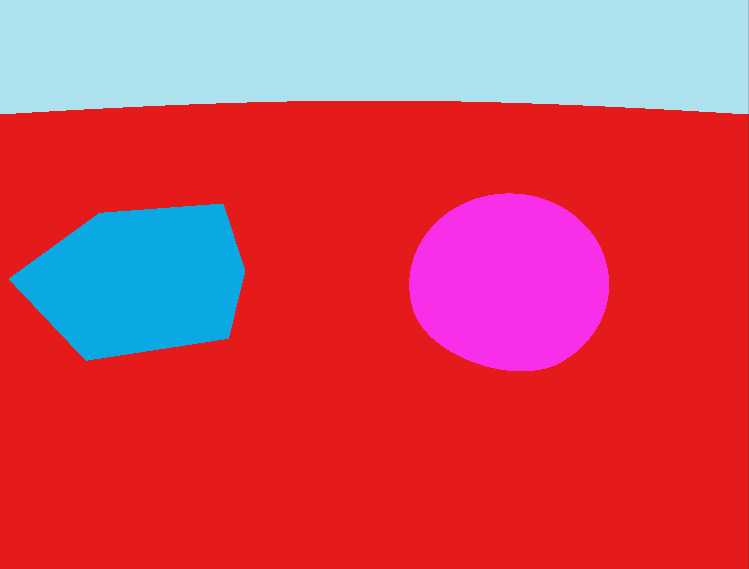
\includegraphics[width=\textwidth]{Plantilla-TFG-master/img/escena1_plana.png}
        \caption{Colores planos}
    \end{subfigure}
    \hfill
    \begin{subfigure}[b]{0.3\textwidth}
        \centering
        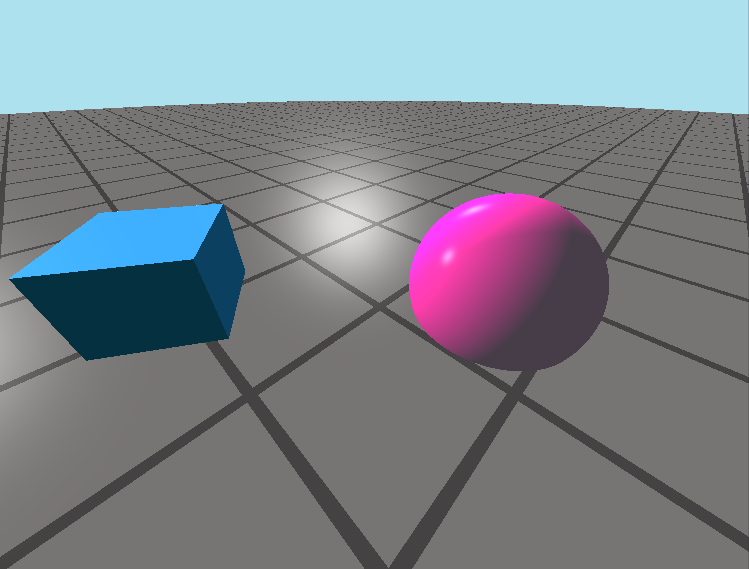
\includegraphics[width=\textwidth]{Plantilla-TFG-master/img/escena2_blinn.png}
        \caption{Modelo de Blinn}
    \end{subfigure}
    \hfill
    \begin{subfigure}[b]{0.3\textwidth}
        \centering
        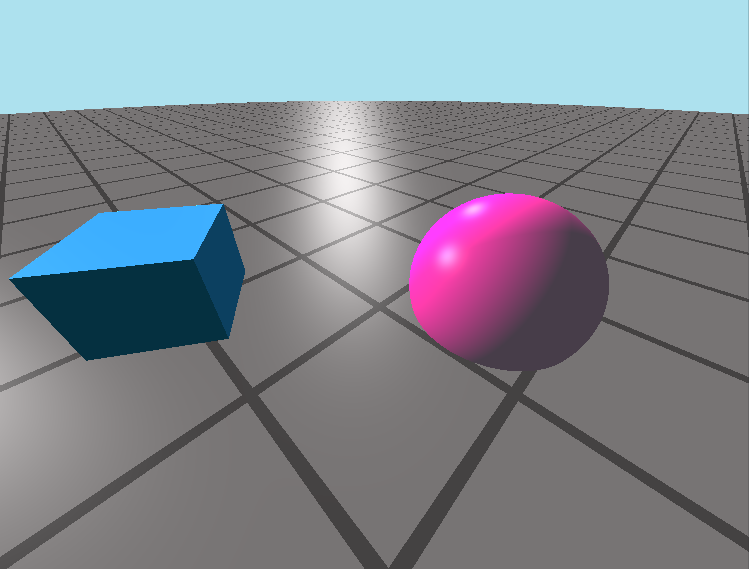
\includegraphics[width=\textwidth]{Plantilla-TFG-master/img/escena3_blinnPhong.png}
        \caption{Modelo de Blinn-Phong}
    \end{subfigure}
    \medskip
    \begin{subfigure}[b]{0.3\textwidth}
        \centering
        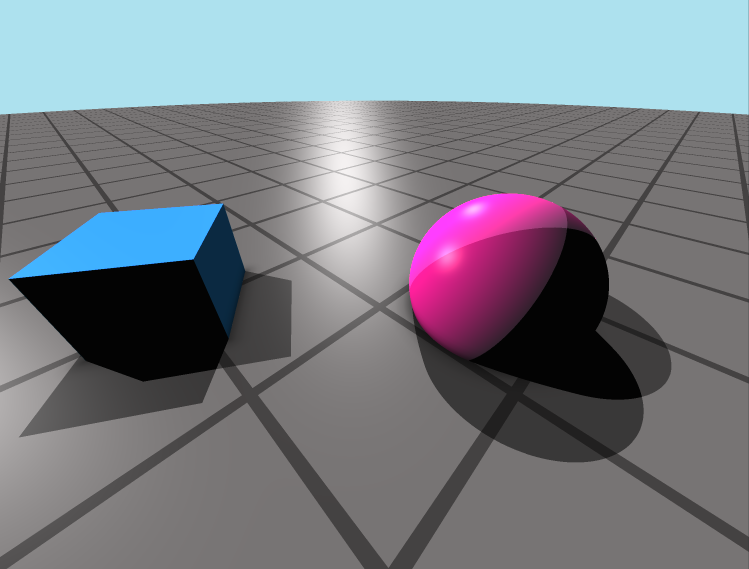
\includegraphics[width=\textwidth]{Plantilla-TFG-master/img/escena4_sombraPlana.png}
        \caption{Sombras planas}
    \end{subfigure}
    \hfill
    \begin{subfigure}[b]{0.3\textwidth}
        \centering
        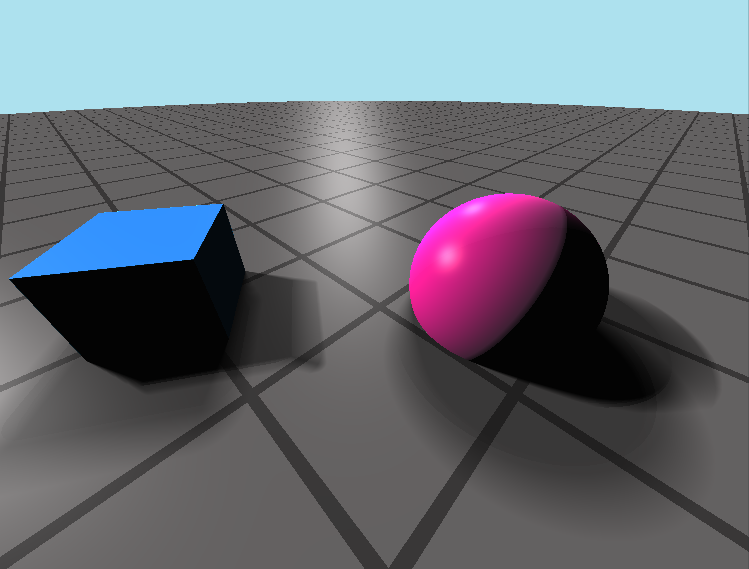
\includegraphics[width=\textwidth]{Plantilla-TFG-master/img/escena5_sombraSuave1.png}
        \caption{Sombras suaves básicas}
    \end{subfigure}
    \hfill
    \begin{subfigure}[b]{0.3\textwidth}
        \centering
        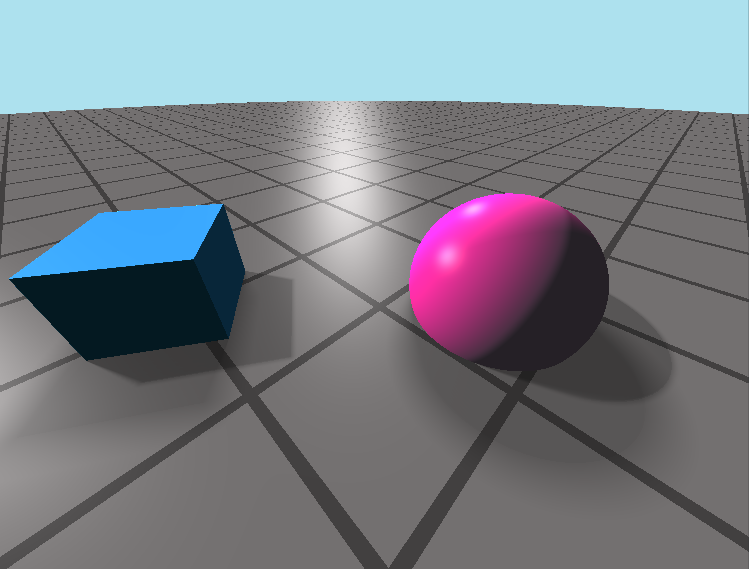
\includegraphics[width=\textwidth]{Plantilla-TFG-master/img/escena6_sombraSuave2.png}
        \caption{Sombras suaves avanzadas}
    \end{subfigure}
    \medskip
    \begin{subfigure}[b]{0.45\textwidth}
        \centering
        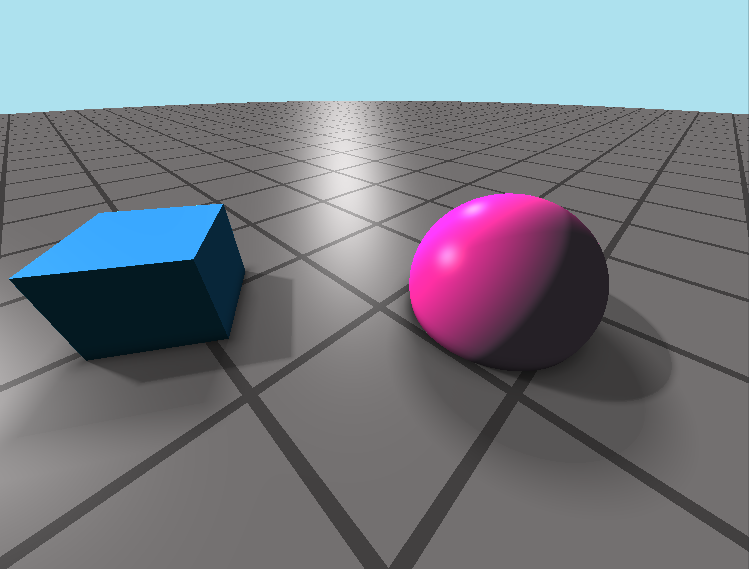
\includegraphics[width=\textwidth]{Plantilla-TFG-master/img/escena7_AO.png}
        \caption{Oclusión ambiental}
    \end{subfigure}
    \hfill
    \begin{subfigure}[b]{0.45\textwidth}
        \centering
        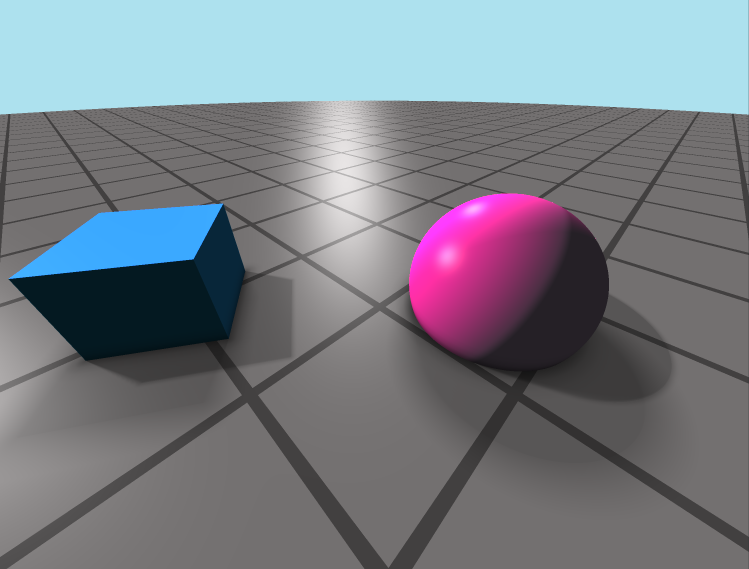
\includegraphics[width=\textwidth]{Plantilla-TFG-master/img/escena9_AA3.png}
        \caption{\textit{Antialiasing}}
    \end{subfigure}

    \caption{Renderizado de SDF añadiendo técnicas de iluminación y renderizado avanzadas}
\end{figure}


\endinput